\subsection{App}

\subsubsection{Verbindungsüberprüfung}

Da die App ohne eine bestehende Internetverbindung nicht sinnvoll nutzbar ist, wird direkt beim öffnen der App überprüft ob eine Verbindung zum SIS-Server (also eine Internetverbindung) besteht.\\
Dazu wird ein Bild vom SIS-Server geladen, dieses wird dann aber ausgeblendet, da es rein zur Verbiundugsüberprüfung dient. Wenn das Bild erfolgreich geladen werden kann heißt das, dass eine Verbindung zum Server besteht. Tritt beim Laden des Bildes ein Fehler auf heißt das, dass die Verbindung zum Server fehlerhaft ist beziehungsweise nicht besteht. In diesem Fall wird, mit Hilfe der alert-Funktion, eine Meldung ausgegeben, dass keine Verbindung aufgebaut  werden konnte.\\

\lstinputlisting[style=custom, language=html, caption={/index.html; Bild laden zur Verbindungsüberprüfung; Zeile 65}, label={lst:widget}, firstline=65, lastline=65, firstnumber=65]{sources/app/index.html}

\subsubsection{Login}

\paragraph{Datenübermittleung\\}
Beim Login müssen als erstes die Anmeldedaten an den Server übertragen werden. Da in der App kein PHP verwendet werden kann werden die Daten über ein iFrame an den Server gesandt.\\

\lstinputlisting[style=custom, language=html, caption={/index.html; Login-Formular; Zeilen 69-81}, label={lst:widget}, firstline=69, lastline=81, firstnumber=69]{sources/app/index.html}

Dadurch dass die login.php im iFrame geladen wird, wird die HTML-Seite nicht neu geladen.\\
Wenn die Daten an den Server gesandt wurden erstellt dieser eine Session für den Benutzer.\\

\paragraph{Überprüfung der Session\\}
	
Da über das iFrame nicht überprüft werden kann ob die Anmeldung korrekt durchgeführt werden konnte, muss noch eine zusätzliche PHP-Datei geladen werden um das zu überprüfen. In dieser PHP-Datei wird überprüft ob eine Session für den Nutzer existiert, falls die Session existiert wird JavaScript-Code ausgegeben, welcher den Nutzer in das Menü der App weiterleiten soll.\\

\lstinputlisting[style=custom, language=php, caption={/mobile/api/checkCookie.php; Überprüfung der Session; Zeilen 1-7}, label={lst:widget}, firstline=1, lastline=7, firstnumber=1]{sources/app/api/checkCookie.php}

Damit der JavaScript-Code ausgeführt werden kann wird diese Datei als JavaScript eingebunden. Da die Überprüfung der Session aber erst nach der Eingabe der Daten durch den Nutzer durchgeführt wird, muss diese Datei dynamisch mit Hilfe von JavaScript eingebunden werden.\\

\lstinputlisting[style=custom, language=html, caption={/index.html; Funktion checkCookie(); Zeilen 14-18}, label={lst:widget}, firstline=14, lastline=18, firstnumber=14]{sources/app/index.html}

Sollte die Anmeldung erfolgreich gewesen sein, wird nun der folgende JavaScript-Code geladen, und leitet den Nutzer in das Menü der App weiter.\\

window.location.href='menu.html';

\paragraph{Automatische Wiederanmeldung\\}
	
Um die Bedienung der App zu erleichtern, wurde die Funktion \enquote{Angemeldet bleiben} integriert. Dadurch wird der Benutzer, falls er diese Funktion bei der letzten Anmeldung ausgewählt hat, beim öffnen der App automatisch angemeldet.\\

Damit das Funktioniert müssen der Benutzername und das Passwort des Nutzers gespeichert werden, diese werden aber nur lokal auf dem Gerät gespeichert und können nicht ausgelesen werden.\\

Um die Daten zu speichern wurde die Funktion saveLogin() erstellt.\\

\lstinputlisting[style=custom, language=html, caption={/index.html; Funktion saveLogin(); Zeilen 32-39}, label={lst:widget}, firstline=32, lastline=39, firstnumber=32]{sources/app/index.html}


Mit der Funktion window.localStorage.setItem() können Variablen oder sonstige Daten auf dem lokalen Speicher des Smartphones gespeichert werden.\\
 Die Funktion saveLogin() wird nach jedem Anmeldeversuch ausgeführt, falls der Benutzer bei Angemeldet bleiben einen Hacken gesetzt hat. Sollte die Anmeldung fehlschlagen, weil ein falscher Benutzername oder ein falsches Passwort eingegeben wurden, werden die Daten sofort wieder gelöscht.\\
Wenn der Benutzer nicht mehr angemeldet bleiben möchte, muss er sich (durch klicken auf den logout-Button) abmelden. Wenn das gemacht wird, wird die Funktion logout() ausgeführt diese leitet den Benutzer zurück auf die Anmeldeseite und löscht Benuzternamen und Passwort.\\

\lstinputlisting[style=custom, language=html, caption={/logout.html; Funktion logout(); Zeilen 8-13}, label={lst:widget}, firstline=8, lastline=13, firstnumber=8]{sources/app/logout.html}

\subsubsection{Konfigurationsdatei-config.xml}

Um die Metadaten der App zu konfigurieren, um bestimmte Einstellungen zu treffen oder um Plugins zu laden wird die Datei config.xml benötigt. Diese Konfigurationsdatei wird zusammen mit allen anderen Dateien in das ZIP-Paket gespeichert und für den PhoneGap build hochgeladen.\\
Die config.xml besteht grundsätzlich aus XML-Code.\\
Am Anfang der Datei steht ein Widget-Tag in welchem die ID der Applikation und die Versionsnummer angegeben werden.\\
 
\lstinputlisting[style=custom, language=xml, caption={/config.xml; App-Basisinformationen; Zeilen 2-6}, label={lst:widget}, firstline=2, lastline=6, firstnumber=2]{sources/app/config.xml}


Weitere Tags sind\\
\begin{description}
\item[\texttt{<name></name>}] Damit wird der Name der App angegeben
\item[\texttt{<description></description>}] Darin wird eine Beschreibung der App geschrieben
\item[\texttt{<author email="help@sis.htlinn.ac.at"></author>}] Zwischen diesen Tags wird angegeben wer die App erstellt hat.
\item[\texttt{<icon src="images/icon.png" />}] Mit diesem Tag kann man den Pfad des App-Icons angeben.
\item[\texttt{<gap:splash src="images/splash.png" />}] Mit diesem Tag kann man den Pfad des Splashscreens angeben.
\item[\texttt{<access origin="http://sis.htlinn.ac.at"/>}]Mit dem Access-Tag gibt man an auf welche Webseiten die App zugreifen, bzw. welche Webseiten die App laden darf.
\item[\texttt{<gap:plugin name=" " version="" />}] Mit diesem Tag werden Plugins eingebunden.
\item[\texttt{<manifest> </manifest>}] Das Manifest Tag wurde verwendet um das Android-Manifest zu erstellen,darin kann man	Berechtigungen für die Android-App einstellen. Das Manifest wäre in diesem Fall aber nicht notwendig gewesen.
\end{description}

Für iOS wird das Icon in vielen verschiedenen Größen benötigt, damit die App für alle Geräte angepasst ist. Darum wurden zusätzlich noch zwölf Icons erstellt und in der config.xml eingebunden. Damit die Icons auch richtig zugewiesen werden, werden dem Icon-Tag noch jeweils ein Attribut für die Höhe und die Breite des Bildes und ein Attribut um das richtige Betriebssystem anzugeben, mitgegeben.\\
Beispiel:\\

\lstinputlisting[style=custom, language=xml, caption={/config.xml; Icon 76px für iOS; Zeile 32}, label={lst:widget}, firstline=32, lastline=32, firstnumber=32]{sources/app/config.xml}
	

Bei den Splashscreens (das Bild das beim Starten der App erscheint) müssen auch mehrere Formate eingebunden werden.
Um zu vermeiden, dass es durch PhoneGap zu Problemen mit der Kommunikation zwischen der App und dem Server kommt wurde die URL des Servers (\href{https://sis.htlinn.ac.at}{https://sis.htlinn.ac.at}), mit Hilfe des Access-Tags als Ausnahme hinzugefügt.\\

Bei den Preferences wurde eingestellt, dass die Applikation keine Berechtigungen hat,\\

\lstinputlisting[style=custom, language=xml, caption={/config.xml; Berechtigungen aufheben; Zeile 84}, label={lst:widget}, firstline=84, lastline=84, firstnumber=84]{sources/app/config.xml}

Dadurch wird beim Installieren der App, die Verbindung mit dem Internet als einzige angeforderte Berechtigung angezeigt. Diese Berechtigung kann bei PhoneGap-Apps nämlich nicht abgestellt werden.\\

Weiters wurde mit den Preferences noch eingestellt, dass die App im Fullscreen-Modus betrieben wird und das die App bevorzugt auf dem externen Speicher installiert wird.\\

\subsubsection{Debugging}
Während der Entwicklung wurde die Applikation nur auf dem PC getestet. Da die App rein aus Webtechnologien aufgebaut wird, kann diese auch im Webbrowser ausgeführt werden.\\
Das betreiben der App auf dem PC zieht einige Vorteile mit sich. Die App muss nicht nach jeder Änderung neu gebuildet und auf das Smartphone geladen werden, sondern kann direkt nach der Änderung des Codes im Webbrowser neu geladen und getestet werden. Des Weiteren hat man im Webbrowser sehr mächtige Werkzeuge um Fehler im Code zu finden, zum Beispiel die Entwicklerkonsole.\\

\subsubsection{Erstellen einer App mit PhoneGap}
Um die App zu erstellen wurde die Onlinevariante von PhoneGap, PhoneGap Build, verwendet. Dazu muss man sich zuerst bei AdobeSystems registrien, das kann man aber kostenlos machen.\\
Danach meldet man sich unter \href{https://build.phonegap.com}{https://build.phonegap.com} an und kommt es erscheint folgende Seite.\\

\begin{figure}[H]
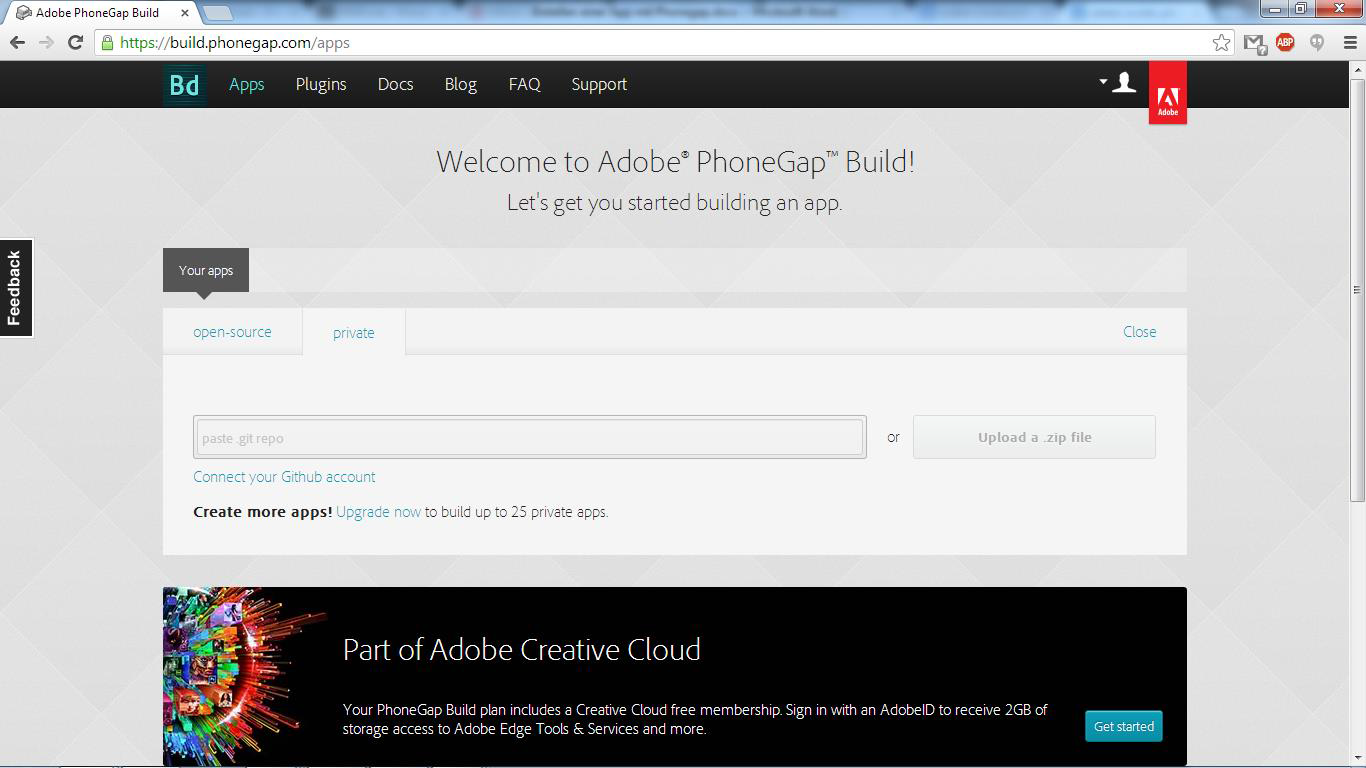
\includegraphics[keepaspectratio=true, width=14cm]{images/phoneGap/PhoneGap1.png}
\caption{PhoneGapwebsite vom 21.04.2014}
\end{figure}

Hier muss man nun den Reiter \enquote{private} auswählen, damit man die Appdaten in Form eines Zipfiles hochladen kann.
Um Fortzufahren, muss man nun das Zipfile, in welchem die Daten für die App(alle HTML, CSS und JavaScript-Files) gespeichert sind, hochladen.\\
Ist das geschehen, versucht die Webseite die Apps für Android, WindowsPhone und iOS zu compilieren. Für Android und WindowsPhone funktioniert das auch, falls der Code und vor allem die Konfigurationsdatei korrekt sind, aber bei iOS kommt eine Fehlermeldung. Denn um Apps für iOS zu erstellen benötigt man Zertifikate, welche man nur als Apple-Developer bekommt.\\
Nach dem ersten Build sieht man, dass für den Appnamen das Appsymbol und weitere Einstellungen die Einstellungen aus der config.xml übernommen wurden.\\

\begin{figure}[H]
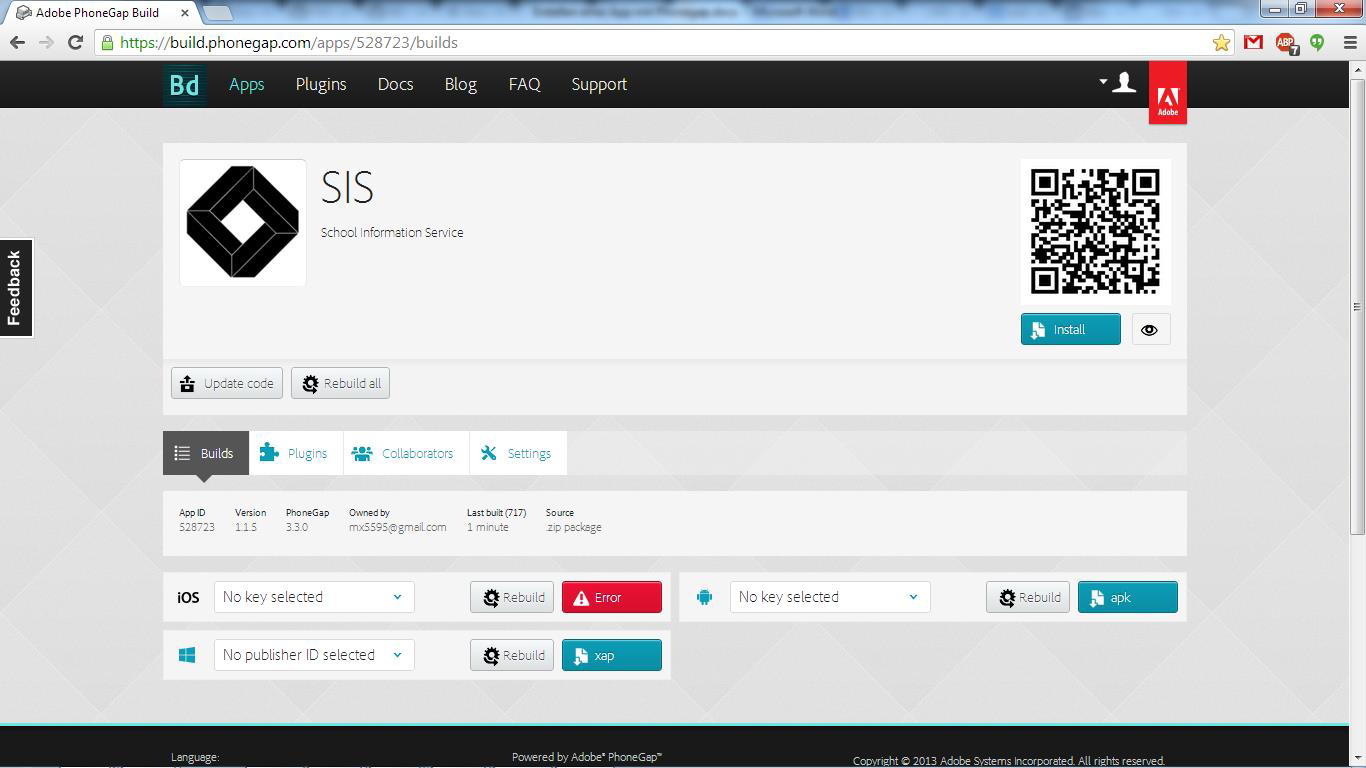
\includegraphics[keepaspectratio=true, width=14cm]{images/phoneGap/PhoneGap2.png}
\caption{PhoneGapwebsite vom 21.04.2014}
\end{figure}

Um die Applikation zu updaten, müssen alle Dateien die verändert wurden in der ZIP-Datei ausgetauscht werden und die ZIP-Datei muss neu hochgeladen werden. Dazu klickt man einfach auf \enquote{Update code} und wählt dann die gewünschte ZIP-Datei aus.\\
Die Android-App und die App für WindowsPhone kann man jetzt bereits testen. Bei Android muss man dazu nur zuerst in den Einstellungen, im Untermenü Anwendungen, die Option \enquote{Unbekannte Quellen} aktivieren. Dann kann man einfach das APK-File auf das Gerät laden(entweder direkt mit dem Gerät downloaden oder via USB, Bluetooth, etc. auf das Gerät laden) und ausführen, und die Applikation wird wie jede andere App installiert. Nun kann man die App nutzen.\\
Die App auf dem WindowsPhone zu nutzen ist etwas umständlicher. Entweder man stellt die App direkt in den Store oder wenn man sie nur testen möchte, kann man die App auch mit Hilfe von Developer Tools direkt auf das Smartphone laden und testen.\\
Damit die Android-App in den Play-Store von Google geladen werden kann, muss diese zuerst noch signiert werden. Dazu muss eine Keystore-Datei erzeugt werden, mit welcher die App signiert werden kann.\\
Dieses Keystore-File kann man selbst erstellen, sofern man die JDK (Java Development Kit) installiert hat. Um den Schlüssel zu erstellen muss man die Eingabeaufforderung öffnen und in das Verzeichnis der JDK wechseln, als nächstes kann man mit dem Befehl keytool und einigen Parametern ein Keystotre-File erstellen.\\
Beispielbefehl:\\

\begin{lstlisting}
keytool -genkey -v -keystore my-release-key.keystore -alias alias_name -keyalg RSA -keysize 2048 -validity 10000
\end{lstlisting}

Nachdem dieser Befehl eingegeben wurde, wird man noch aufgefordert, den Namen des Entwicklers oder Entwicklerteams, die Nationalität und einige weiter Angaben einzugeben. Zuletzt muss noch ein Passwort angegeben werden, dieses wird benötigt um den Schlüssel zu entsperren, wenn er bei PhoneGap genutzt wird.\\
Nun wird eine Datei, in diesem Fall mit dem Namen my-release-key.keystore, erstellt.\\
Wenn man nun das Dropdownmenü neben dem Androidsymbol öffnet,\\

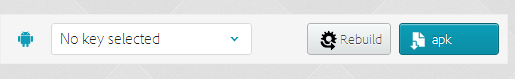
\includegraphics[keepaspectratio=true, width=7cm]{images/phoneGap/PhoneGap3.png}

erscheint ein Punkt \enquote{add a key…}. Wenn man diesen Punkt auswählt wird man aufgefordert eine Datei hochzuladen, dabei handelt es sich um die Keystore-Datei, welche zuvor erzeugt wurde. Dann muss man dem Schlüssel noch einen Namen geben und bestätigen.\\
Nun kann man in diesem Dropdownmenü den hochgeladenen Schlüssel auswählen, um ihn zu nutzen muss man zuerst noch ein Passwort eingeben, das ist jenes Passwort welches zuvor beim erstellen des Keystore-Files angegeben wurde. Wenn man nun einen Rebuild macht, bekommt man eine Android-Release-App, welche auch im Play-Store veröffentlicht werden kann.
Bei iOS benötigt es bereits ein Entwicklerzertifikat, um eine Debug-App zu erstellen. Um ein solches Zertifikat zu erstellen muss man bei Apple als Developer angemeldet sein und 99\$ im Jahr bezahlen.\\
Für dieses Projekt wurde der Apple-Enterprise-Account der Schule genutzt. Man benötigt nur eine Apple ID (Registrierung unter \href{https://developer.apple.com/register/}{https://developer.apple.com/register/} ), mit dieser kann man dann von einem Administrator (in unserem Fall Direktor Laner) zum Account hinzugefügt werden.\\
Nachdem man zum Enterprise-Programm hinzugefügt wurde, muss man das MemberCenter (https://developer.apple.com/membercenter/ ) öffnen.\\

\begin{figure}[H]
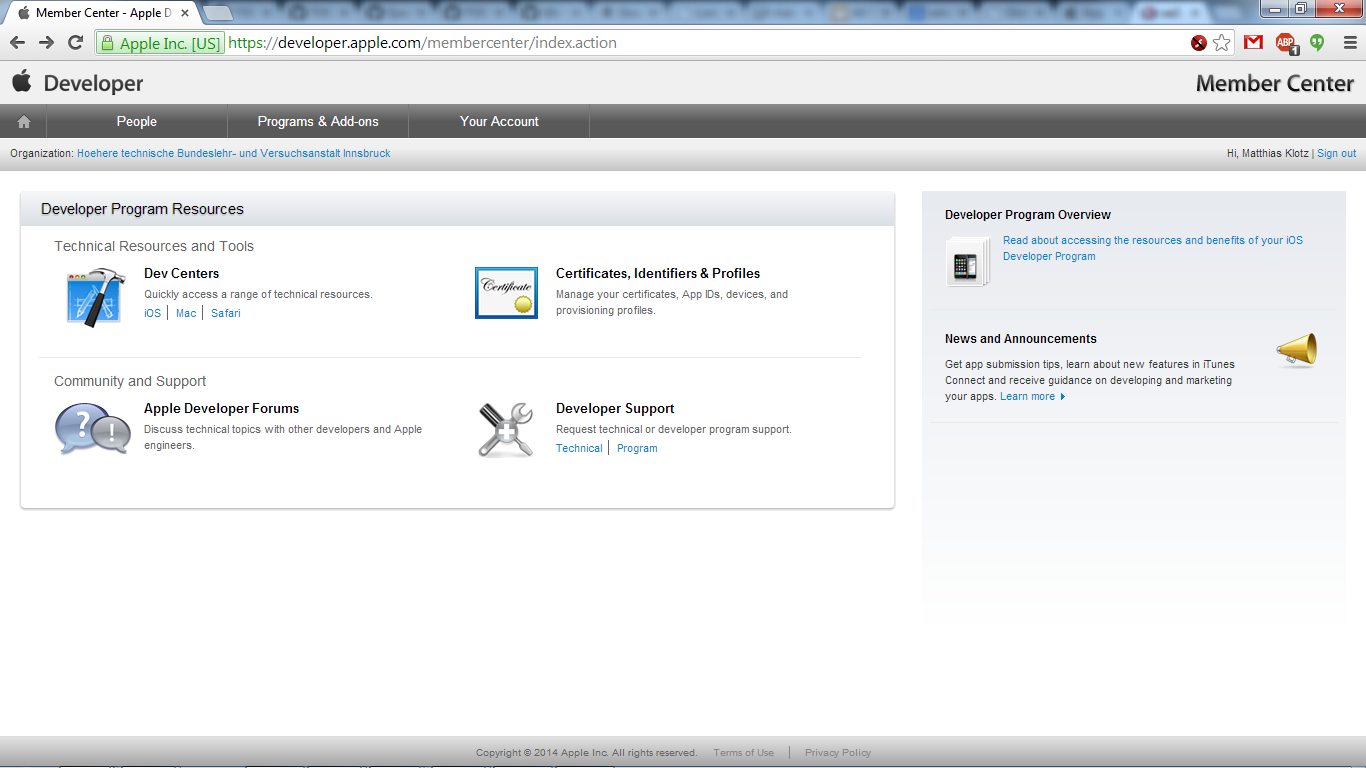
\includegraphics[keepaspectratio=true, width=14cm]{images/phoneGap/AppleMemberCenter1.png}
\caption{Applewebsite vom 21.04.2014}
\end{figure}

Unter \enquote{Certificates, Indentifiers \& Profiles} kann man nun die benötigten Zertifikate erstellen und downloaden.\\

\begin{figure}[H]
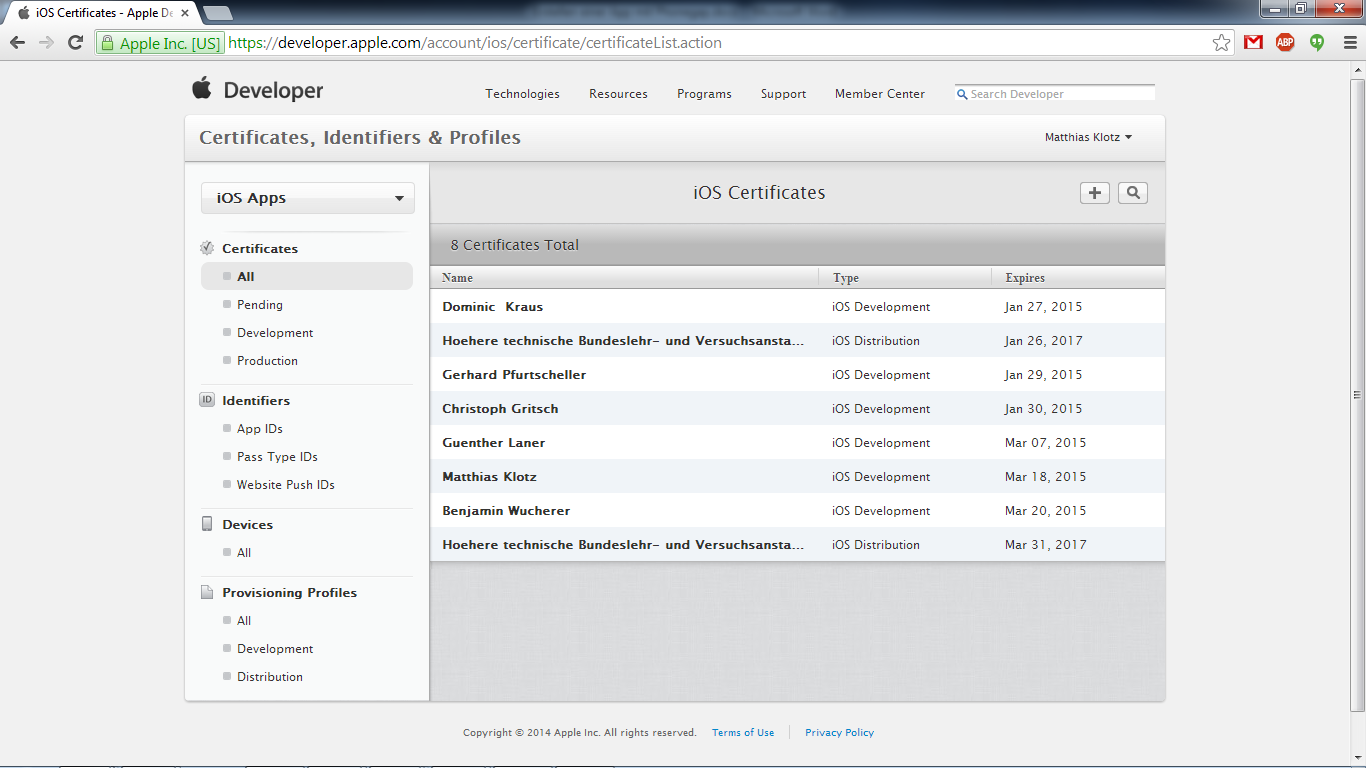
\includegraphics[keepaspectratio=true, width=14cm]{images/phoneGap/AppleMemberCenter2.png}
\caption{Applewebsite vom 21.04.2014}
\end{figure}

Um ein neues Zertifikat zu erstellen, öffnet man zuerst den Menüpunkt Certificates und klickt dann auf das Plus-Symbol in der rechten oberen Ecke des Fensters. Daraufhin erscheint der Assistent zum erstellen eines neuen Zertifikates.
Als erstes wird gefragt wozu das Zertifikat verwendet wird. Dabei muss man zuerst unterscheiden ob es sich um ein Development oder ein Production Zertifikat handelt. Bei einem Development Zertifikat
werden bestimmte Developergeräte angegeben, auf welchen die Applikation getestet werden kann, ohne dass sich die App im Appstore befindet.\\
Ein Production Zertifikat wird hingegen benötigt, um eine App zu erstellen, welche für alle Geräte nutzbar ist, diese App muss dann aber für gewöhnlich über den Appstore veröffentlicht werden.\\
Für dieses Projekt wurden beide Varianten erstellt und genutzt.\\
Bei beiden Varianten wird man im nächsten Schritt aufgefordert einen CSR (Certificate Signing Request) hochzuladen. Diese \enquote{Datei} erhält man indem man die Schlüsselbundverwaltung bei Mac OS X öffnet und im Menü Datei unter Zertifikats Assistent, \enquote{neues Zertifikat erstellen} wählt. Dabei wird man aufgefordert eine E-Mail-Adresse und den eigenen Namen anzugeben, wichtig ist das der Punkt als Datei speichern ausgewählt wird.\\
Nach Angabe der Informationen kann man nun eine CSR-Datei abspeichern. Diese Datei wird als nächstes bei der Erstellung des Zertifikates auf der Apple-Website hochgeladen. Nun kann man das Zertifikat erstellen und downloaden.
Als nächstes muss noch ein Provisoining-File erstellt werden. Dazu wechselt man einfach auf den Menüpunkt Provisioning Profiles und klickt dann auf das selbe Symbol wie zuvor bei den Zertifikaten. Es erscheint wieder ein Assistent, der bei der Erstellung des Provisioning Profils hilft. Als erstes muss man wieder angeben wozu das Provisioning Profile benötigt wird. Wenn man zuvor ein Development Zertifikat erstellt hat, muss man nun wieder Development auswählen, hat man aber zuvor ein Production Zertifikat erstellt, muss man nun Distribution auswählen. Im nächsten Schritt muss noch eine App-ID gewählt werden, dazu wurde einfach eine bereits existierende ID ausgewählt. Als nächstes wird nach einem Zertifikat gefragt, hier wird das zuvor erstellte Zertifikat ausgewählt.\\
Falls ein Development Provisioning Profile erstellt wird, wird man noch nach den Entwicklergeräten gefragt, hier muss man sein eigenes iPhone, welches zuvor unter Devices hinzugefügt wurde, auswählen.\\
Wenn man soweit ist kann man auch das Provisioning Profile generieren und herunterladen.\\
Da für PhoneGap aber ein privater Schlüssel in Form eines P12-Files benötigt wird, muss dieser erst aus dem Zertifikat exportiert werden. Dazu muss man zuerst das heruntergeladene Zertifikat in die Schlüsselbundverwaltung importieren, dann wählt man das soeben importierte Zertifikat aus, nun klickt man mit der rechten Maustaste darauf und wählt exportieren aus und exportiert das Zertifikat als P12-Datei.\\
\\
Wenn man nun das Dropdownmenü neben dem Apple-Logo öffnet,

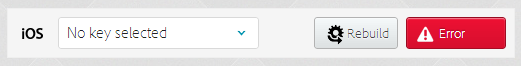
\includegraphics[keepaspectratio=true, width=7cm]{images/phoneGap/PhoneGap4.png}

erscheint ein Punkt \enquote{add a key…}. Wenn man diesen Punkt auswählt wird man aufgefordert zwei Dateien hochzuladen, eine P12-Datei und ein Provisioning-File, dabei handelt es sich um die beiden Dateien die gerad erstellt wurden. Wenn diese Dateien hochgeladen wurden kann die Applikation erstellt werden.\\
Hat man ein Developer-Zertifikat erstellt, kann die erstellte App nur auf den in dem Zertifikat bestimmten Geräten betrieben werden, wurde aber ein Distribution Zertifikat erstellt, kann die App nun auf allen iOS-Geräten verwendet werden.\\
Um die App für den App-Store zu builden, wurden uns die Zertifikate von Direktor Günther Laner zur Verfügung gestellt, da die Applikation über den Developer Account des Direktors veröffentlicht wird.\\



\subsubsection{Veröffentlichen der App}

Apps werden meistens in verschiedenen Stores zur Verfügung gestellt. iOS Apps im iTunes-Store von Apple, Android Apps im Play-Store von Google und WindowsPhone Apps im WindowsPhone-Store.\\
\paragraph{Android\\}
Die Android App wurde anfangs nicht über den Play-Store verbreitet, sondern wurde auf der SIS-Homepage als Download zur Verfügung gestellt. Es wurde einfach die APK-Datei als Download zur Verfügung gestellt und auf jedem Gerät welches Unbekannte Installationsquellen zulässt konnte die App installiert werden.\\
Um die Applikation in dem gewünschten Store zu veröffentlichen muss zuerst ein Release-APK erzeugt werden. Dazu muss die App signiert werden, dafür gibt es bei PhoneGap die Möglichkeit ein Keysotre-File hochzuladen. \\
Um Apps im Play-Store zu veröffentlichen, muss man bei Google als Developer registriert sein. Dazu benötigt man nur einen normalen Google-Account (z.B. eine GMail-Adresse), unter \href{https://developer.android.com}{https://developer.android.com} wählt man dann den Reiter Distribution aus.\\

\begin{figure}[H]
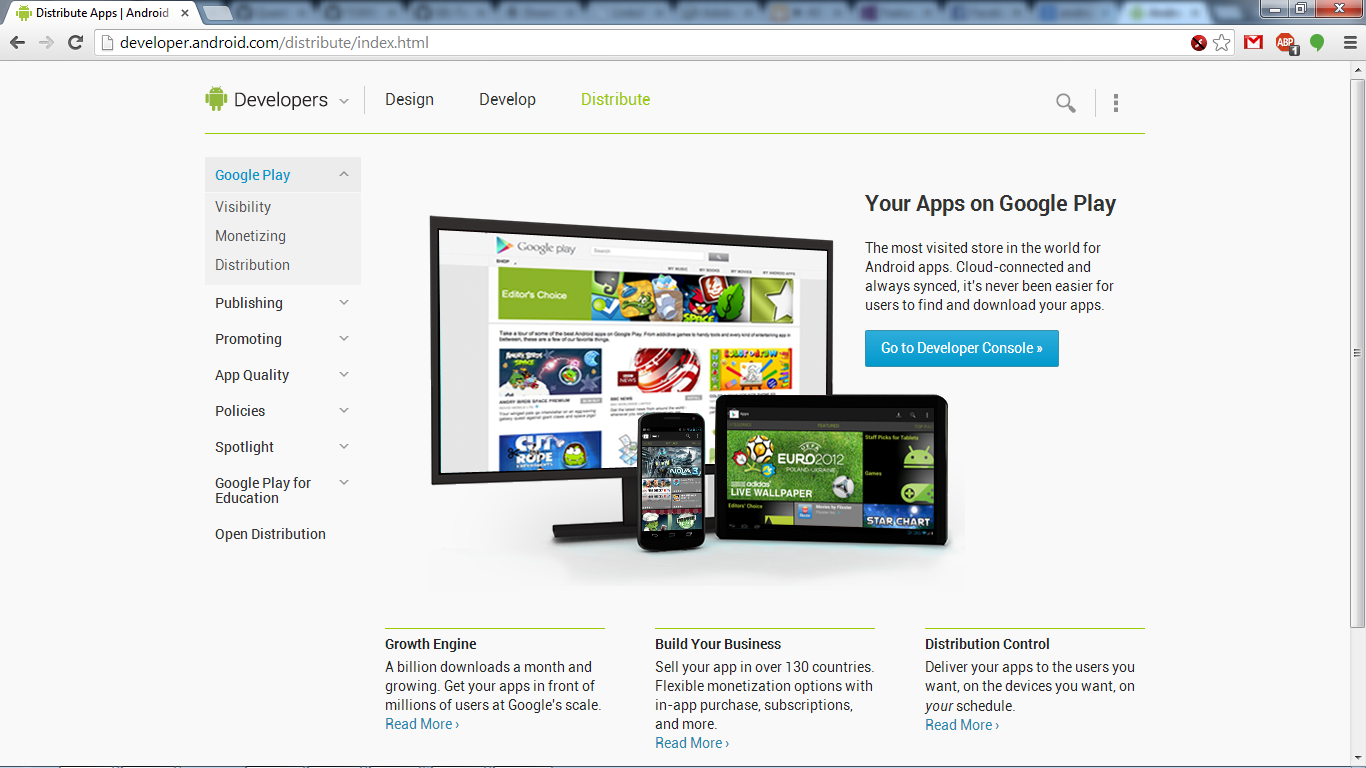
\includegraphics[keepaspectratio=true, width=14cm]{images/appstores/AndroidDeveloper1.png}
\caption{Android Developer Webseite vom 21.04.2014}
\end{figure}

Nun wählt man \enquote{Go to Developer Console >>} aus. Man wird zu einer Seite weitergeleitet, auf welcher man den Account mit welchem man angemeldet ist, als Developer-Account registrieren kann. Das kostet jedoch einmalig 25\$, für das Veröffentlichen einer App muss nichts mehr gezahlt werden.\\
Für dieses Projekt wurde der Google Account von Professor Stecher verwendet und die Registrierungsgebühr wurde von der Schule bezahlt.\\
Wenn man als Developer registriert ist muss man wieder auf \enquote{Go to Developer Console >>} klicken, dann kommt man zur Developer Konsole, wo man Apps hochladen und bearbeiten kann.\\

\begin{figure}[H]
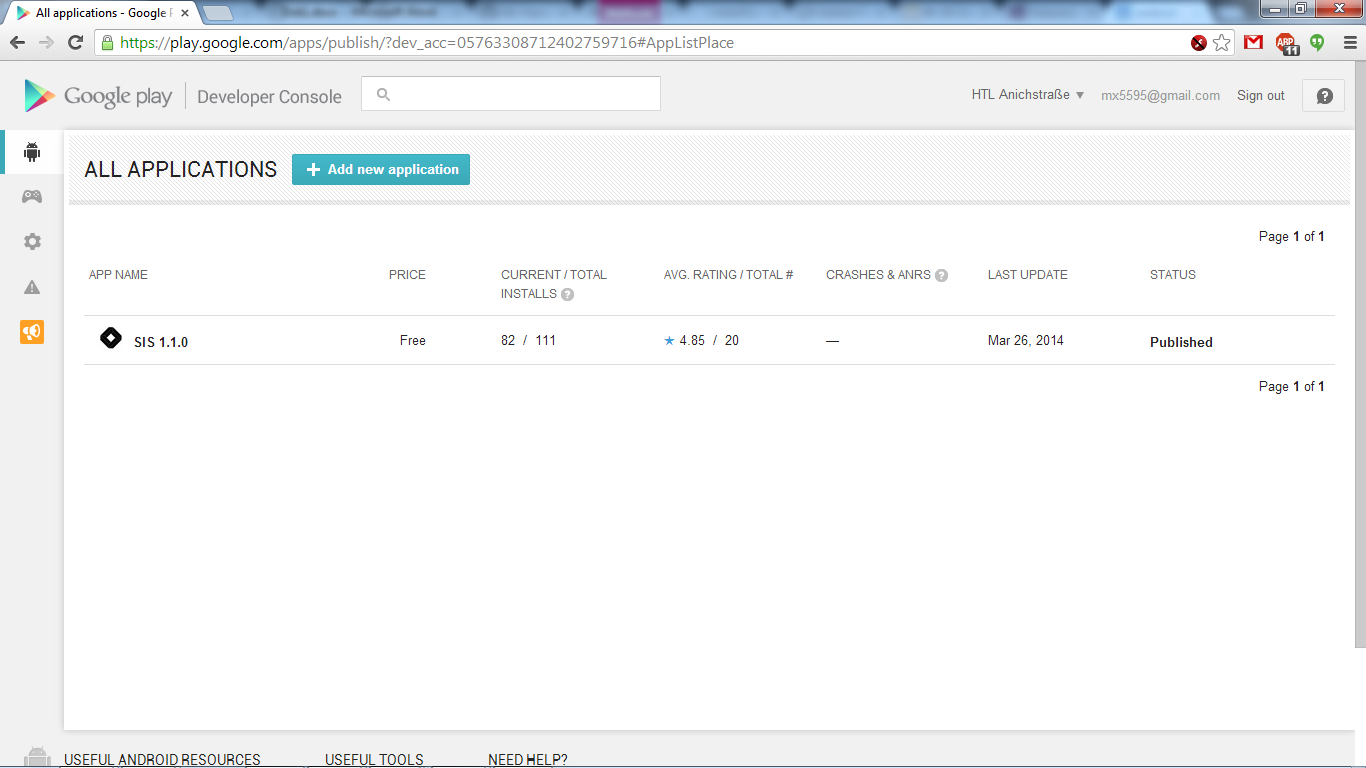
\includegraphics[keepaspectratio=true, width=14cm]{images/appstores/AndroidDeveloper2.png}
\caption{Android Developer Webseite vom 21.04.2014}
\end{figure}

Durch klicken auf \enquote{Add new application} kann man eine neue App hochladen. Dazu muss man nur die Release-APK welche zuvor von PhoneGap heruntergeladen wurde, hochgeladen werden. Danach muss man noch eine kurze Beschreibung der App angeben und Screenshot hochladen. Zusätzlich muss noch angegeben werden in welchen Ländern die App verfügbar ist und dass die App kostenfrei erhältlich ist.\\
Wenn alle Einstellungen getroffen wurden, kann man die App veröffentlichen. Nun wird die App noch von Google überprüft und nach wenigen Stunden erscheint die App, falls keine Probleme auftreten, im Play-Store.\\

\paragraph{WindowsPhone\\}

Um die WindowsPhone App zu veröffentlichen muss man bei Microsoft als Developer registriert sein. Dazu benötigt man zuerst einen Microsoft-Account (z.B. eine Outlook.com E-Mail-Adresse), dann kann man sich auf dieser Seite \href{https://dev.windowsphone.com/en-us/join}{https://dev.windowsphone.com/en-us/join}  als WindowsPhone-Developer registrieren, das kostet ca. 17\$ jährlich.\\
Für die Veröffentlichung der App wurde der Microsoft Account von Fachlehrer Hilpold verwendet, welcher sich freundlicherweise als Developer registrierte.\\
Nun wählt man auf der Seite \href{https://dev.windowsphone.com/}{https://dev.windowsphone.com/} den Punkt\enquote{Submit apps} aus. Auf der Seite auf welche man nun weitergeleitet wird, kann man die App in Form eines XAP-Files hochladen. Zusätzlich müssen noch Screenshots eingefügt werden und es muss eine Beschreibung der App in der richtigen Sprache abgegeben werden.\\

\paragraph{iOS\\}

Bei iOS wurde auch eine Möglichkeit gefunden den iTunes App Store anfangs zu umgehen und die App über einen anderen Weg zu veröffentlichen bis die App im App Store ist. PhoneGap bietet die Möglichkeit, die App direkt auf dem iPhone zu installieren. Dazu muss man nur die Downloadseite (QR-Code-Link) mit dem iPhone laden und PhoneGap fragt automatisch nach ob die App installiert werden soll.\\
Die Veröffentlichung der App im iTunes-Store wurde von der Tochter des Direktors, Frau Karin Laner übernommen, daher sind mir nur die Anforderungen an die Applikation bekannt welche von Apple gestellt werden damit diese veröffentlicht werden kann.\\
Folgende Informationen werden benötigt um die Applikation in den iTunes Store hochzuladen:\\
• die Installationsdatei welch von PhoneGap heruntergeladen wurde (IPA-Datei)\\
text:\\
• App Name\\
• bundle display name (name below icon on the iPhone)\\
• version number\\
• copyright\\
• primary category\\
• secondary category (optional)\\
• rating (any offensive material that requires 12+ rating?, see below)\\
• free or paid app?\\
• available in all territories or only certain ones (which countries?)\\
• available in only German or other languages as well?\\
• description (in all languages)\\
• keywords (for search in app store)\\
• support URL\\
• contact information\\
• any encryption within the app?\\
• any 3rd party content within the app?\\
files for app store:\\
• app icon for app store (1024 x 1024 px)\\
• screenshots:\\
• 1-5 screenshots for 3,5 inch iPhone: 640 x 960 px\\
• 1-5 screenshots for 4 inch iPhone: 640 x 1136 px\\
files within xcode project folder:\\
• all referenced libraries / frameworks if externals used\\
• icon\\
• 57 x 57 px - Icon.png\\
• 114 x 114 px - Icon@2x.png\\
• 120 x 120 px - Icon-60@2x.png\\
• 29 x 29 px - Icon-Small.png\\
• 58 x 58 px - Icon-Small@2x.png\\
• 80 x 80 px - Icon-Small-40@2x.png\\
• Default (loading) asset:\\
• 320 x 480 px - Default.png\\
• 640 x 960 px - Default@2x.png\\
• 640 x 1136 px - Default-568h@2x.png\\
• 640 x 960 px - iOS7-Default@2x.png\\
• 640 x 1136 px - iOS7-Default-568h@2x.png\\
\\
All diese Informationen und Daten wurden an Frau Karin Laner weitergeleitet, welche sich dann um die weiteren Schritte der Veröffentlichung kümmerte.\\

% Hier dürfen auch auch Sourcecode-Teile vorkommen.
% Wenn Sourcecodes: jeweilge File in den Ordner /sources/ in einen Unterordner packen und mit folgendem Befehl includieren:
%
%
% \lstinputlisting[style=custom, language=php, caption={Dateiname}, label={lst:content_imple_timetables_labelname}]{sources/ordner/datei.php}
%
% Als weitere Eigenschaft kannst du die Zeilen angeben: [firstline=300, lastline=500]
% Damit nicht alles reinkopiert wird.